% ACL format. Camera/arXiv build: latexmk -pdf main.tex
% Anonymous build:                 latexmk -pdf -jobname=main_review -pdflatex='pdflatex %O "\def\REVIEW{1}\input{%S}"' main.tex
% Figures 2-5: python figures.py (numbers copied from the report files named there).
\documentclass[11pt]{article}
\ifdefined\REVIEW
  \usepackage[review]{acl}
\else
  \usepackage[]{acl}
\fi
\newcommand{\codeavail}{\ifdefined\REVIEW the supplementary material\else \url{https://github.com/vedant-jumle/Seahorse}\fi}
\usepackage{times}
\usepackage{latexsym}
\usepackage[T1]{fontenc}
\usepackage[utf8]{inputenc}
\usepackage{microtype}
\usepackage{graphicx}
\usepackage{url}
\usepackage{amsmath,amssymb}
\usepackage{booktabs}
\usepackage{multirow}
\usepackage{xcolor}
\usepackage{tikz}
\usepackage{placeins}
\usetikzlibrary{arrows.meta,positioning,calc,fit}

\newcommand{\ci}[2]{\,{\scriptsize[#1,\,#2]}}
\newcommand{\cond}[1]{\textsc{#1}}

\title{What Binds a Memory? Cache Slices, Recurrent States,\\and Why Separately Stored Facts Swap}

\author{Vedant Jumle \\
  Delft University of Technology \\
  \texttt{vvjumle@student.tudelft.nl}}

\begin{document}
\maketitle

\begin{abstract}
A fact a user states in one conversation can be carried into the next by storing part of the model's own key/value
cache and putting it back later. We ask which part carries the fact, and what goes wrong when several such memories
are used together. On three frozen models (Qwen2.5-1.5B, the hybrid Qwen3.5-2B and Llama-3.2-3B), the answer reads a
stated fact from the value's own position, late in the network, so writing a state at the subject cannot work. Two
stored positions (the value and the full stop after it; on the hybrid, with its recurrent state) restore 0.87--1.00 clean use against 0.90--1.00 with the
sentence in context, while the same two tokens as text give 0.24--0.27. On the hybrid, the two kinds of memory
dissociate: the recurrent state recognises a name it is shown (yes/no 0.93) but cannot choose between two (0.48), and
the attention entries choose (0.91) but cannot verify (0.50). Attention entries alone also refuse direct questions,
and a generic ``answer personal questions'' direction removes most of that refusal. Slices stored in separate
sessions swap partners when used together (partner confusion 0.33--0.41), because every one of them was encoded as
the first fact of its conversation: storing a new memory as the second fact cuts confusion to 0.09--0.15, joint
encoding writes the binding at the subject's positions, and storing the $k$-th memory as the $k$-th fact works for
three memories but only halves the swaps for five, where neighbouring order tags blur.
\end{abstract}

\begin{figure*}[t]
\centering
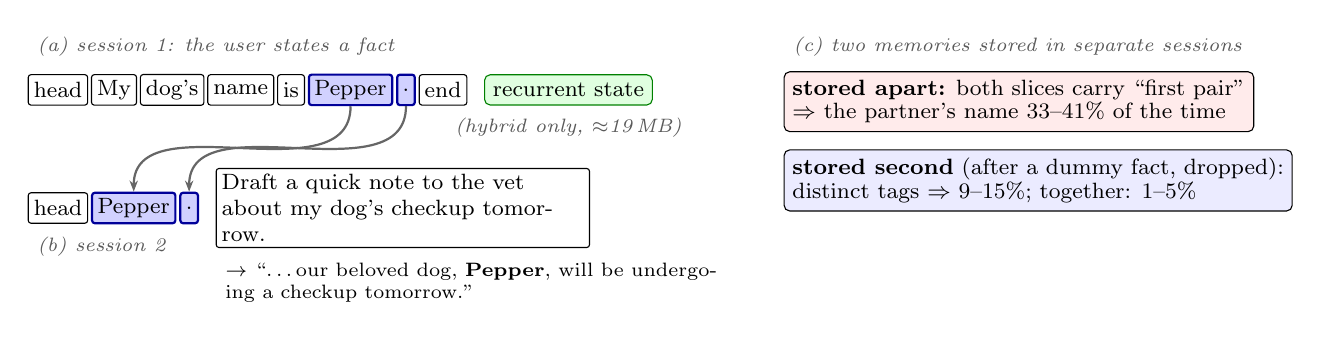
\begin{tikzpicture}[font=\footnotesize, tok/.style={draw, rounded corners=1pt, inner sep=2pt, minimum height=11pt},
  kept/.style={tok, fill=blue!18, draw=blue!60!black, thick}, lbl/.style={font=\scriptsize\itshape, text=black!65},
  arr/.style={-{Stealth[length=4pt]}, thick, black!60}]
% (a) session 1
\node[lbl, anchor=west] (la) at (0,1.15) {(a) session 1: the user states a fact};
\node[tok, anchor=west] (h1) at (0,0.6) {head};
\node[tok, right=1pt of h1] (u1) {My};
\node[tok, right=1pt of u1] (u2) {dog's};
\node[tok, right=1pt of u2] (u3) {name};
\node[tok, right=1pt of u3] (u4) {is};
\node[kept, right=1pt of u4] (v) {Pepper};
\node[kept, right=1pt of v] (fs) {.};
\node[tok, right=1pt of fs] (eot) {end};
\node[draw=green!50!black, fill=green!12, rounded corners=2pt, right=6pt of eot, inner sep=3pt] (st) {recurrent state};
\node[lbl, below=1pt of st, align=center] {(hybrid only, $\approx$19\,MB)};
% (b) session 2
\node[lbl, anchor=north west] at (0,-1.15) {(b) session 2};
\node[tok, anchor=west] (h2) at (0,-0.9) {head};
\node[kept, right=1pt of h2] (v2) {Pepper};
\node[kept, right=1pt of v2] (fs2) {.};
\node[tok, right=6pt of fs2, align=left, text width=4.6cm] (q) {Draft a quick note to the vet about my dog's checkup tomorrow.};
\node[anchor=north west, align=left, font=\scriptsize, text width=6.2cm] (a) at ($(q.south west)+(0,-2pt)$)
  {$\rightarrow$ ``\dots our beloved dog, \textbf{Pepper}, will be undergoing a checkup tomorrow.''};
\draw[arr] (v.south) to[out=-90, in=90] (v2.north);
\draw[arr] (fs.south) to[out=-90, in=90] (fs2.north);
% (c) collision
\node[lbl, anchor=west] at (9.6,1.15) {(c) two memories stored in separate sessions};
\node[draw, rounded corners=2pt, anchor=west, fill=red!8, align=left, inner sep=3pt] (c1) at (9.6,0.45)
  {\textbf{stored apart:} both slices carry ``first pair''\\[-1pt]$\Rightarrow$ the partner's name 33--41\% of the time};
\node[draw, rounded corners=2pt, anchor=west, fill=blue!8, align=left, inner sep=3pt] (c2) at (9.6,-0.55)
  {\textbf{stored second} (after a dummy fact, dropped):\\[-1pt]distinct tags $\Rightarrow$ 9--15\%; together: 1--5\%};
\end{tikzpicture}
\caption{\textbf{(a--b)} A fact stated in session~1 is carried into session~2 by keeping the model's own keys and
values at two positions, the value and the full stop after it (blue), and, on a hybrid model, the recurrent state
after the turn; they are reinstated as a user-turn segment before a later question when its subject matches.
\textbf{(c)} Slices stored in separate sessions were each encoded as the first fact of their conversation, and swap
partners when used together; storing the new one as the second fact removes most swaps (\S\ref{sec:two}).}
\label{fig:main}
\end{figure*}

\section{Introduction}
\label{sec:intro}

What has to be stored for a fact a user stated in one conversation to be \emph{used} in a later one? Text retrieval
answers by storing the words and re-reading them \citep{lewis2020rag,packer2023memgpt}. Weight editing stores an
association in the MLPs \citep{meng2022rome,meng2023memit}. A third option keeps something from the model's own
forward pass. Our earlier work stored the activation change an experience causes and added it back later as a
steering vector \citep{jumle2026steering}: the change carried leanings, but facts came out only as the word to say,
almost never used in a sentence (at most 0.15 clean use against 0.96--0.98 in context). A pushed vector is one
direction at one position, and in-context binding works through positions: the model binds an attribute to its entity
with a shared order tag and fetches the attribute from its own position when asked
\citep{feng2024binding,prakash2024entity,prakash2026lookbacks,dai2024binding}.

This paper asks what a stored representation needs in order to be read by those circuits, using the model's own key/value
cache as the store. Reinstating a cached turn is prompt caching \citep{gim2024promptcache}; systems work reuses
cached chunks for speed \citep{yao2025cacheblend,hu2025epic,xiao2024infllm}. Our question is different: which part of
the cache carries a fact, what a hybrid model's recurrent state adds, and why combining separately stored memories
fails. Everything is training-free, on frozen models, with pre-registered decision rules (\S\ref{sec:setup}).

\paragraph{Contributions.}
\begin{itemize}\setlength\itemsep{0pt}
\item \textbf{What carries a fact} (\S\ref{sec:carry}). The answer reads a stated value from the value's own position,
late; the subject holds no copy. Two stored positions, the value and the full stop after it, restore the fact in a
new session (0.87--1.00 clean use on three models), far beyond the same tokens as text (0.24--0.27).
\item \textbf{What a hybrid's two memories do} (\S\ref{sec:hybrid}). On Qwen3.5-2B the recurrent state recognises a
name it is shown and rejects look-alike names, but cannot choose between two names; the attention entries choose but
cannot verify, and refuse direct questions. That refusal is mostly a generic response gate, not a memory-specific
signal.
\item \textbf{Why separately stored facts swap, and a cheap fix} (\S\ref{sec:two}). Every separately stored slice was
encoded as the first fact of its conversation. Storing a new memory as a later fact removes most swaps without
re-encoding; joint encoding writes the binding at the subject's positions; the fix works for three memories and halves
the swaps for five.
\end{itemize}

\section{Setup}
\label{sec:setup}

\paragraph{Models.} Qwen2.5-1.5B-Instruct \citep{qwen2024qwen25} and Llama-3.2-3B-Instruct \citep{grattafiori2024llama3},
both full attention, and Qwen3.5-2B \citep{qwen2026omni}, a hybrid with full attention in 6 of its 24 blocks and Gated
DeltaNet \citep{yang2025gdn} in the other 18. Qwen3.5-9B is used teacher-forced only (Appendix~\ref{app:9b}). All in
fp32, frozen.

\paragraph{Facts.} A memory is one sentence the user said, e.g.\ \textit{``My dog's name is Pepper.''} We use 7
hand-written facts (pet, family and work names) and 52 more drawn from a pool (30 people, 8 pets, 14 attributes such as
a hometown). Each fact has \emph{use} prompts (two per hand-written fact, one templated per pool fact) that need it without asking for it (\textit{``Draft a quick note to the vet about my dog's checkup tomorrow''}), a \emph{direct} question (\textit{``What's my dog's name?''}) and balanced
yes/no probes (\textit{``Is my dog called Pepper?''} vs.\ an unrelated name).

\paragraph{Harvest and reinstate.} Session~1 is the model's chat template with the sentence as the user turn. We keep
its keys and values (K,V) at chosen positions, and on the hybrid the recurrent and convolution states after the turn.
In session~2, the kept entries are placed as a segment after the template head and before the new user turn, with keys
re-rotated to their new positions; the recurrent state, if kept, initialises the DeltaNet blocks. A gate puts the
memory in only when the question's subject matches the stored subject string; with the gate, the answers to 50
unrelated prompts are token-identical to no memory (1.000 in every gated condition). Table~\ref{tab:conds} lists the
conditions. Reinstating the whole turn reproduces the sentence as an earlier user turn exactly (max $|\Delta|$ logit
$\le 1.1{\times}10^{-4}$), which every run checks.

\begin{table}[t]
\centering\small
\begin{tabular}{@{}ll@{}}
\toprule
condition & what session 2 contains \\
\midrule
\cond{ctx} & the sentence in the user turn (ceiling) \\
\cond{nomem} & nothing (floor) \\
full-turn slice & K,V of the whole stored turn \\
2-position slice & K,V at the value and the full stop \\
same tokens as text & ``Pepper.'' as an earlier user turn \\
\midrule
\multicolumn{2}{@{}l}{\textit{hybrid (Qwen3.5-2B): which parts of the memory}} \\
attention entries & 2 positions, 6 attention blocks \\
recurrent state & the DeltaNet state only, no K,V \\
both & 2 positions + the state \\
\bottomrule
\end{tabular}
\caption{Conditions for one memory. Two-memory conditions are in \S\ref{sec:two}.}
\label{tab:conds}
\end{table}

\paragraph{Measures.} Each prompt is answered once greedily and with four samples. \emph{Clean use} means the answer
uses the stored value correctly and is coherent, by the majority of three judges from different families (Qwen3.5-9B,
gpt-oss and Gemma-4; a tie goes to the first). Teacher-forced measures read $\Delta\log P$ of the value at the answer
prefix (\textit{``Your dog's name is''}) and the yes/no margin at the first answer token. Intervals are 95\% bootstrap
CIs over items, then prompts (2000 resamples); differences are paired.

\paragraph{Pre-registration.} The first experiments (where the value is read, the subject write, the slice
conditions) were pre-registered with decisive rules; every later part was added as an addendum with its rule written
and committed before any job ran. We report each rule's verdict, including the ones that fail
(Appendix~\ref{app:prereg}). Code, rules and reports: \codeavail.

\section{What carries a fact}
\label{sec:carry}

\paragraph{The value is read from its own position.} Patching the question's subject token between two facts moves at
most 0.02 of the answer's preference, at every block and on all three models; patching the stored value moves all of
it (1.00). Blocking the answer's attention to the value in Qwen2.5's last five blocks removes 0.59 of the gain; the
rest reaches the answer through other positions, mainly the full stop. This is the in-context route
\citep{prakash2026lookbacks,feng2024binding} rather than enrichment at the subject \citep{geva2023dissecting}, and it
rules out a write at the subject: storing the subject's enriched state and adding it back gives 0.00 clean use.

\paragraph{Two positions are enough.} Figure~\ref{fig:carry} shows clean use on the use prompts. Keeping only the
value and the full stop gives 0.87 on Qwen2.5 (the sentence in context: 0.90), 1.00 on Llama (1.00) and, with the
recurrent state, 0.97 on the 2B (1.00). A slice harvested after an unrelated exchange still works (0.80 on Qwen2.5,
1.00 on Llama), and on the 52 pool facts the 2-position slice reaches 0.97 (Qwen2.5) and 0.98 (Llama) on use prompts.
Because the slice sits in a user-turn segment, the model treats the fact as the user's (on Qwen2.5 it never claims
the fact as its own), unlike a steering vector \citep{jumle2026steering}.

\begin{figure}[t]
\centering
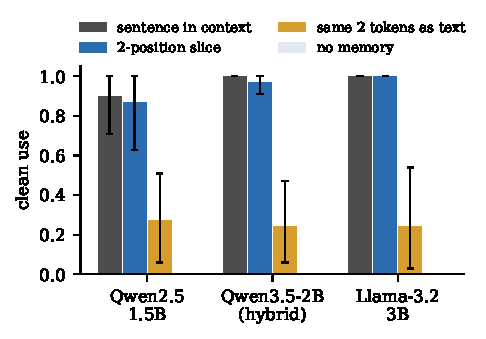
\includegraphics[width=\columnwidth]{figures/fig2.pdf}
\caption{Clean use on the use prompts of the 7 hand-written facts. The 2-position slice (on the 2B with the recurrent
state) is close to the sentence in context; the same two tokens as text are not.}
\label{fig:carry}
\end{figure}

\paragraph{The slice carries more than its tokens.} The same two tokens as an earlier user turn (\textit{``Pepper.''})
give 0.27, 0.24 and 0.24 (Figure~\ref{fig:carry}; the slice minus the text $+0.60$ to $+0.76$, all CIs above 0). The
stored K,V at ``Pepper'' and ``.'' were computed with the whole sentence in view, so they carry its relation to the
subject; as text, the model has to guess what ``Pepper'' refers to. The difference also holds for verification: on
Llama, asked \textit{``Is my dog called Pepper or Max?''}, the slice picks the right name 0.95 of the time and the text
0.68.

\section{What a hybrid's two memories do}
\label{sec:hybrid}

On Qwen3.5-2B the attention entries and the recurrent state can be kept separately. Teacher-forced, the 2-position
attention entries alone carry the value ($\Delta\log P$ $+10.0$ nats; in context $+10.65$), the state alone only part
of it ($+4.2$). In generation the attention entries alone give 0.67 clean use on use prompts but refuse direct
questions (\textit{``I don't know your dog's name! Could you tell me what it is?''}), and the state alone gives no recall at all (0.00).

\paragraph{The state recognises; the attention entries select.} Two question forms separate the parts
(Figure~\ref{fig:hybrid}). Asked \textit{``Is my dog called Pepper?''}, the state alone answers correctly 0.93 of the
time (balanced against unrelated names), the attention entries alone 0.50 (always ``No''). Asked \textit{``Is my dog
called Pepper or Max?''}, the order reverses: attention entries 0.91, state 0.48. The state signals that a name it is
shown was said; the attention entries can pick out which name it was but not confirm it. The recognition sits in the
recurrent state, not the convolution buffer (yes/no 0.86 vs.\ 0.50).

\begin{figure}[t]
\centering
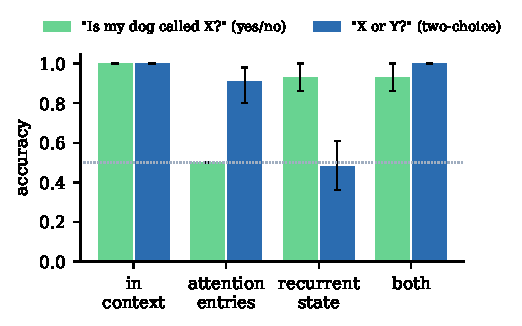
\includegraphics[width=\columnwidth]{figures/fig3.pdf}
\caption{Qwen3.5-2B, 7 facts, teacher-forced. The recurrent state verifies a name it is shown but cannot choose
between two; the attention entries choose but cannot verify. Dotted: chance.}
\label{fig:hybrid}
\end{figure}

\paragraph{Recognition is of the item, and it does not bind.} \citet{afendulev2026hybrid} find, within one session
on Qwen3.5, that the recurrent state supports recognition but also accepts associated lures, a gist familiarity. Across
sessions, our state alone rejects lures more often than unrelated names: false ``yes'' 0.00 for look-alike names
(Pepper/Piper) and 0.04 for same-theme names (Pepper/Ginger) against 0.07 for unrelated ones (balanced accuracy against
lures 0.96\ci{0.88}{1.00}); on 38 pool facts, look-alike minus unrelated is $-0.01$\ci{-0.05}{0.03} (balanced 0.94).
The pre-registered verdict is item recognition both times. But the joint state of two facts says yes to either name
for either person (balanced 0.50\ci{0.40}{0.60}): it records which names were said, not whose they are.

\paragraph{Why the attention entries refuse.} The value is there, so the refusal is a decision to answer. A
difference-of-means ``told'' direction (the sentence in context minus no memory, at the last prompt token, built on
other facts) restores direct answers from the attention entries (Table~\ref{tab:refusal}); a random direction of the
same norm and the reversed sign do not, and the told direction without a memory makes the model invent a name rather
than recall one. But a \emph{comply} direction built with no memory at all, from personal questions the model refuses
(\textit{``What's my blood type?''}) minus matched general ones (\textit{``What's the most common blood type?''}), does
most of the same job (cosine with told 0.4--0.65 in the middle and late blocks). On the 2B the told direction beats it
by only $+0.09$\ci{0.00}{0.18}, so the pre-registered verdict is ``generic comply''; on Qwen2.5 ($+0.09$\ci{0.03}{0.15})
and Llama ($+0.15$\ci{0.07}{0.25}) a small told-specific part remains. On held-out facts the told direction also lowers
use-prompt clean use on the 2B and Qwen2.5 ($-0.14$, $-0.18$), which comply does not. The attention-only refusal is
thus mostly the model's generic refusal of personal questions, close to the refusal direction of
\citet{arditi2024refusal}; the recurrent state lifts it in a way that is partly item-specific (own entries with
another fact's state 0.65, with a placebo sentence's state 0.60, with its own 0.88).

\begin{table}[t]
\centering\small
\setlength{\tabcolsep}{4pt}
\begin{tabular}{@{}lccc@{}}
\toprule
direct question, clean use & Qwen2.5 & 2B & Llama \\
\midrule
attention-only slice ($X$) & 0.72 & 0.12 & 0.62 \\
$X$ + told & 0.89 & 0.76 & 0.88 \\
$X$ + told, random dir. & 0.72 & 0.15 & 0.64 \\
$X$ + told, reversed & 0.17 & 0.09 & 0.49 \\
$X$ + comply (no memory) & 0.80 & 0.67 & 0.73 \\
$X$ + comply, random dir. & 0.59 & 0.12 & 0.51 \\
no memory + told & 0.00 & 0.03 & 0.00 \\
\midrule
use prompts: $X$ $\to$ $X$+told & .98$\to$.80 & .68$\to$.54 & .99$\to$.98 \\
\bottomrule
\end{tabular}
\caption{Refusal of direct questions on 26 held-out pool facts (directions built on the other 26). $X$ = the
2-position slice (on the 2B, attention entries only).}
\label{tab:refusal}
\end{table}

\section{Two or more memories}
\label{sec:two}

\paragraph{Separately stored slices swap partners.} Two facts are stored in separate sessions and both slices are put
back before a question about one of them (gates forced open). With 8 hand-written pairs, 5 of them confusable (two
members of one kind, e.g.\ a first and a second dog) and 3 with different subjects, the answer gives the partner's
name instead of the member's own in 0.37 (Qwen2.5), 0.33 (2B) and 0.41 (Llama) of confusable answers, against 0.01--0.05
when the two sentences were encoded together (Figure~\ref{fig:collide}). Different subjects swap too (0.20--0.26).
Placing the second slice after the first, rather than at overlapping positions, does not help, and on the 2B the
swaps persist with the joint recurrent state, so they arise in the attention entries. On 34 pool pairs the same holds
on all three models (0.16--0.22 vs.\ 0.00).

\paragraph{The cause is storage order.} Binding IDs explain the swap if both slices carry the same ID
\citep{feng2024binding}: each was encoded as the first and only fact of its conversation. We test this directly. The
second member B is harvested after a dummy fact in the same turn (\textit{``My gardener's name is Brian. My second dog's name is Rocky.''}) and the dummy's tokens are dropped, so B's kept tokens are the same tokens as before (asserted)
but were computed as the second fact. Confusion falls from 0.37/0.33/0.41 to 0.09/0.15/0.09, and on the pool pairs to
0.01 on every model, close to joint encoding. Two controls qualify this. An unrelated sentence before B (\textit{``By
the way, I had a coffee this morning.''}) helps less (0.26/0.19/0.31; pool 0.07/0.05/0.13): the effect is not only
that B is no longer at the start of its context, the reading of separately encoded chunks in position-independent
caching \citep{hu2025epic,liu2026hypic}. And storing \emph{both} members second, which should restore the shared tag,
brings the swaps back only on Qwen2.5's pool pairs (0.20 vs.\ 0.22), and only partly elsewhere (0.03--0.21). The
pre-registered rule, which required that, holds on Qwen2.5, on the 2B's hand-written pairs only, and not on Llama.
Storage order explains most of the swaps; a smaller part is generic.

\begin{figure*}[t]
\centering
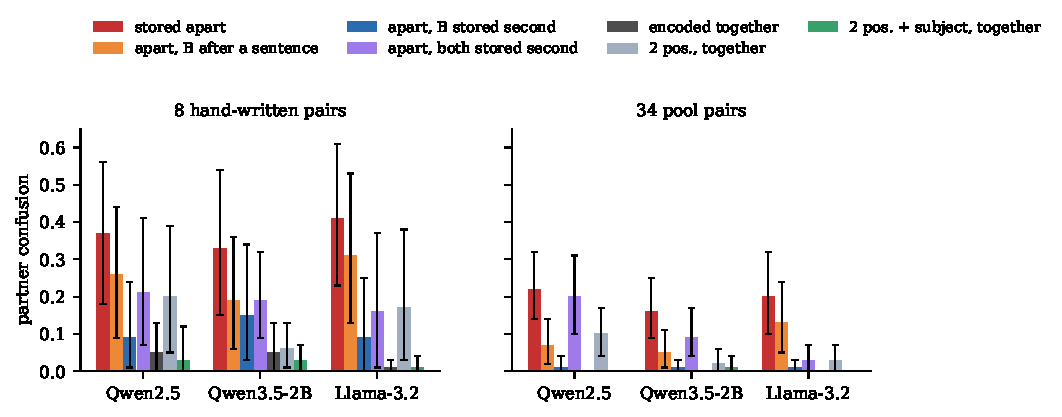
\includegraphics[width=\textwidth]{figures/fig4.pdf}
\caption{Partner confusion (the partner's value in the answer, the member's own not) for confusable pairs, gates
forced open. Storing the second memory as the second fact (blue) removes most swaps; an unrelated sentence before it
helps less; two positions encoded together stay confused on the full-attention models unless the subject's positions
are kept too (green). On the 2B every condition uses the joint recurrent state.}
\label{fig:collide}
\end{figure*}

\paragraph{Joint encoding writes the binding at the subject.} Two stored positions per fact stay confused even when
encoded together (0.20 on Qwen2.5, 0.17 on Llama), so the binding is not at the value. Adding the stored sentence's
subject span (\textit{``younger sister''}, \textit{``friend from work''}) from the joint encoding gives joint
encoding's result (0.03 and 0.01; pool pairs 0.00), while the same positions from separate encodings do not help
(0.34, 0.29). The entity side of the pair's tag is written at the subject's positions, and only when the facts are read
together. On the 2B the joint recurrent state already separates two-position slices (0.06).

\paragraph{The fix scales to three memories, not five.} Storing the $k$-th memory of a set after $k{-}1$ dummy facts
makes it the $k$-th fact (Figure~\ref{fig:scale}). For three same-kind memories (eldest, middle and youngest sister;
first to third dog) confusion falls from 0.47/0.38/0.41 to 0.09/0.04/0.09, against 0.00--0.01 for joint encoding; the
pre-registered rule holds on Qwen2.5 and the 2B and misses on Llama by its overlap clause. For five same-kind pets it
falls from 0.51--0.55 to 0.22--0.30 (joint 0.00--0.03), and the remaining errors are between neighbours: they
concentrate at positions 3 to 5, and the fourth pet is answered with the fifth's or the third's name. Close binding IDs
are confused \citep{feng2024binding}, and the IDs of later positions are closer. For memories about different
subjects, storage order reaches joint encoding at both sizes on all three models (0.00--0.03). Placing the ordered
slices in reverse order changes nothing ($-0.02$ to $+0.03$): what counts is the order a memory was stored in, not
where its slice is put back.

\begin{figure*}[t]
\centering
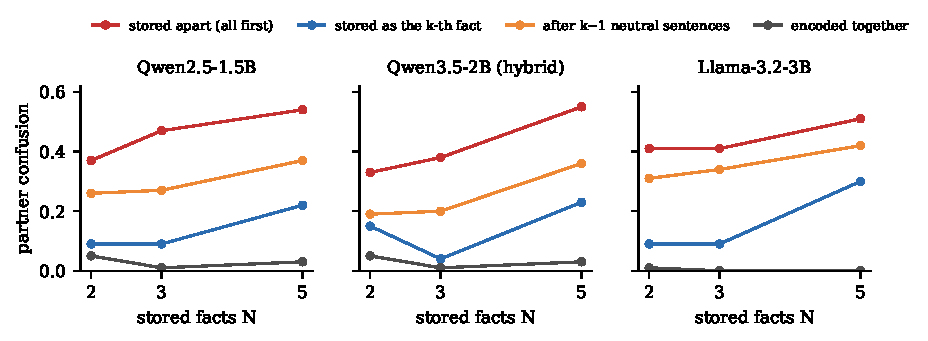
\includegraphics[width=\textwidth]{figures/fig5.pdf}
\caption{Partner confusion against the number of same-kind memories used together (N = 2: the hand-written pairs;
N = 3, 5: 12 and 8 groups). Storing the $k$-th memory as the $k$-th fact tracks joint encoding up to three and
diverges at five.}
\label{fig:scale}
\end{figure*}

\section{Related work}
\label{sec:related}

\paragraph{Binding in context.} Language models bind entities to attributes with binding IDs that are not tied to
position, and confuse IDs that are close \citep{feng2024binding,dai2024binding}; answers are fetched from the
attribute's position through order-ID lookbacks \citep{prakash2024entity,prakash2026lookbacks}. Facts from the weights
are instead enriched at the subject \citep{geva2023dissecting}. We find the in-context route for facts said in an
earlier session, show that separately cached facts share an ID, and locate the entity side at the subject's positions.

\paragraph{Cache reuse.} Prompt Cache reuses separately encoded modules and notes that independence between them
matters \citep{gim2024promptcache}; CacheBlend, EPIC, Hypic and LinearKV recompute part of each reused chunk to
recover the cross-chunk attention it lacks
\citep{yao2025cacheblend,hu2025epic,liu2026hypic,liu2026linearkv}; InfLLM retrieves cached blocks
\citep{xiao2024infllm}; KV-State Grafting restores full cached blocks across sessions \citep{schelpe2026grafting}.
These works measure speed and task accuracy. We measure which part of a cached fact carries it, why separately cached
facts swap, and that a storage-time order fixes it for small sets without recompute.

\paragraph{Hybrid states.} On hybrids, the attention cache carries retrieval and the recurrent state matters little for
it \citep{yu2026dasc}; \citet{afendulev2026hybrid} show recognition from the recurrent state within one session, as
gist familiarity. We show item-specific recognition across sessions and its double dissociation from selection by the
attention entries.

\paragraph{Trained and steered memories.} Cartridges train a small KV cache per corpus
\citep{eyuboglu2026cartridges}; Memory Inception inserts text-derived KV at chosen layers for steering
\citep{liu2026inception}; FwPKM trains a fast-weight memory \citep{zhao2026fwpkm}. Steering vectors as memory carry
leanings but not facts \citep{jumle2026steering}. Known-entity and refusal directions
\citep{ferrando2025entity,arditi2024refusal} bear on why attention-only memories refuse.

\section{Limitations}
\label{sec:limits}

The models are small (1.5--3B in generation; 9B teacher-forced only), and the 2B is the only hybrid tested in
generation. Memories are single sentences about names and simple attributes; we do not test long episodes,
paraphrased questions beyond our prompts, or facts that must be combined. The two-memory results use oracle gates;
retrieval by the subject's words works for 59 facts but turns a wrong pick into a confident wrong answer
(Appendix~\ref{app:retrieval}). Judges are models, checked against each other rather than against human labels. Most
results come from addenda with rules fixed before the run, not from the first pre-registration, and several of their
rules failed in part; we report those verdicts as they came out. The storage-order fix needs to know how many memories
of a set exist, and fails for five same-kind memories, where joint encoding is still needed.

\section{Conclusion}

A stated fact lives at its own position, and a two-position slice of the model's own cache carries it into a new
conversation better than the same words do. On a hybrid, recognition and selection are split between the recurrent
state and the attention entries. The main failure, swaps between separately stored memories, comes from storage
order: every memory thinks it is the first fact. Giving each memory a different place in a stored sequence, or
re-reading the memories that are used together, is work that an offline consolidation phase can do and plain retrieval
over text does not.

\bibliography{refs}

\appendix

\section{Pre-registered rules and verdicts}
\label{app:prereg}

\begin{table*}[t]
\centering\small
\resizebox{\textwidth}{!}{\begin{tabular}{@{}p{0.42\textwidth}lll@{}}
\toprule
rule & models & verdict & where \\
\midrule
Value read at the subject (stage 0, patch + knockout) & Qwen2.5, 2B & pointer-suspected (not at subject) & initial \\
Subject write gives clean use & Qwen2.5 & fails (0.00) & initial \\
Reinstatement wins over the subject write & Qwen2.5 & holds & arm R \\
Slice $>$ text (2-position slice $-$ same tokens, CI $>0$) & all three & holds & add.\ 5, 7 \\
Separately stored facts collide (sep $-$ joint confusion, CI $>0$) & all three & holds (8 and 34 pairs) & add.\ 5, 7, 8 \\
Cheap repair by the binding-ID direction & Qwen2.5 & fails & add.\ 6 \\
State recognition is item recognition, not gist & 2B & holds (7 and 38 facts) & add.\ 7, 8 \\
Missing told signal & 2B / Qwen2.5 / Llama & holds (add.\ 7); held out: fails / fails / holds & add.\ 7, 8 \\
Told is specific vs.\ comply (held out) & 2B / Qwen2.5 / Llama & generic comply / specific / specific & add.\ 8 \\
Pool gap is a prompt-type mismatch & Qwen2.5, Llama & holds & add.\ 7 \\
The 2B value/verification split replicates on the 9B & 9B & fails (strong ``No'' prior) & add.\ 7 \\
Cheap re-encode of the new memory only (2 positions) & all three & fails & add.\ 7 \\
The tag causes the swaps (stored second; both second $\approx$ apart) & Qwen2.5 / 2B / Llama & holds / partly / fails & add.\ 8 \\
The entity side carries the tag (2 positions + subject) & Qwen2.5, Llama & holds & add.\ 8 \\
Two-choice verification usable on Llama & Llama & holds & add.\ 8 \\
Storage order scales, confusable, N = 3 & Qwen2.5 / 2B / Llama & holds / holds / fails (overlap) & add.\ 9 \\
Storage order scales, confusable, N = 5 & all three & fails & add.\ 9 \\
\bottomrule
\end{tabular}}
\caption{Decision rules, in the order they were committed. ``add.'' = an addendum to the pre-registration, written
and committed before its jobs ran. One verdict printed by our report code was corrected by hand: the 2B's told vs.\
comply lower bound was $4{\times}10^{-18}$, printed as ``$>0$''; by the rule's order the verdict is ``generic
comply''. Later rules treat $|\text{bound}|<10^{-9}$ as 0.}
\label{tab:prereg}
\end{table*}

Table~\ref{tab:prereg} lists every decision rule behind a claim in the paper, with its verdict. A judge-pipeline bug
left some answers with only the first judge's label (identical answers across models were judged once and keyed to the
first model); after the fix every answer has all three labels, and no verdict changed (clean use moved by at most 0.02).

\section{Qwen3.5-9B, teacher-forced}
\label{app:9b}

On the 9B the attention entries alone carry the value ($+9.83$ nats; in context $+10.80$) with yes/no at chance, as on
the 2B. The state alone never moves the true name's yes/no margin above zero: the 9B says ``No'' to anything it does
not know (margin about $-3.9$), and the state raises the true name's margin to $-1.27$ against $-3.15$ for unrelated
names and $-3.2$ to $-3.3$ for lures. The margins show item-specific recognition (about $+2.6$ nats on the true name,
$+0.7$ on foils) too weak to overturn the prior, so the binary rule fails.

\section{Retrieval and the binding-ID repair}
\label{app:retrieval}

With slices keyed on the subject's words, the right slice is found for 0.85--0.92 of direct questions at 10, 20 and
59 stored facts on Qwen2.5 (a whole-text key: 0.42--0.61), and the gate fires on unrelated prompts 0--4\% of the time.
A wrong pick is worse than none: the model states the wrong fact with confidence. Separately, a difference-of-means
binding-ID direction is real in the late blocks (it flips which partner the model prefers in 0.75 of held-out
contexts, a random direction 0), but adding it to one stored slice does not reduce swaps in generation
($-0.02$\ci{-0.14}{0.11}).

\section{Example answers}
\label{app:examples}

\begin{itemize}\setlength\itemsep{1pt}
\item 2-position slice, Qwen2.5, \textit{``Draft a quick note to the vet about my dog's checkup tomorrow''}:
\textit{``Subject: Checkup for Pepper, Our Family's Pet. Dear [Vet's Name], I hope this message finds you well. I am
writing to inform you that our beloved dog, Pepper, will be undergoing a checkup tomorrow.\ldots''}
\item Attention entries only, 2B, \textit{``Do you remember my sister's name?''}: \textit{``I don't have access to
personal information about your family members, including your sister's name. As an AI, I don't have the ability to
remember past conversations\ldots''}
\item Attention entries + told, 2B: \textit{``Your ferret's name is \textbf{Shadow}.''}; + comply: \textit{``The name of
your coworker is \textbf{Chloe}.''}
\item No memory + told, 2B: \textit{``Your dentist's name is \textbf{Dr.\ Sarah Jenkins}.''} (invented).
\item Five stored pets, the fourth asked: \textit{``Your fourth cat's name is Atlas.''} (Atlas is the fifth cat).
\end{itemize}

\end{document}
